\chapter{Serverová časť}
Hlavnou funkcionalitou tejto časti je obslúžiť požiadavky prichádzajúce ako http volania, spracovať ich a vrátiť výsledok vo formáte JSON. Backend sa teda priamo nestará o obslúženie užívateľských akcií a ani o routovanie, ale len odpovedá na volania od klienta. V REST API vystavujeme tieto metódy:

 \begin{minipage}{0.9\linewidth}
 	\centering
 	\missingfigure[figheight=10cm]{tabulka rest api}
 	%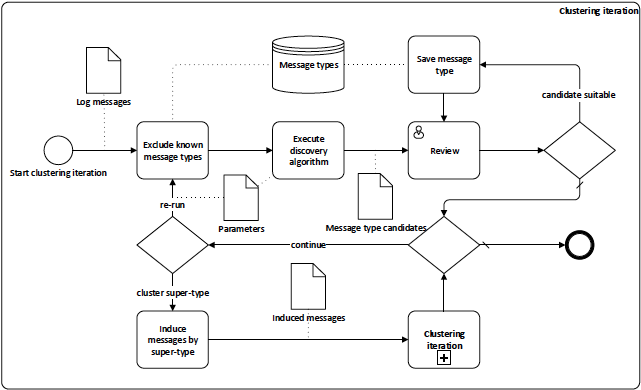
\includegraphics[width=\textwidth]{images/RURC.png} 	
 \end{minipage}
 

Pri implementácii sme sa intenzívne spoliehali na framework Django.
\par Django obsahuje veľké množstvo modulov, z ktorých sme v našej práci síce využili len malú podmnožinu, ktorá nám ale zásadne zjednodušila celú implementáciu. Funkcionalita je rozdelená do samostatných súborov alebo modulov pre jednoduchý a prehľadný kód.

\subsection{Django ORM}
Pre prístup k dátam z databázy je v celej aplikácii použité objektovo-relačné mapovanie zakomponované priamo v Djangu.
\par Využitie Django ORM vo väčšine prípadov vývojára úplne odprostí od potreby implementovať DAL -- Data Access Layer, čiže vrstvu pre prístup k dátam, ako je obvyklé napr. v jazykoch Java alebo C\#. Django ORM používa potomkov triedy \emph{django.db.models.Model}, ďalej nazývaných ako modely, na zadefinovanie štruktúry dát a pôsobí ako jediný prístupový bod k dátam. Každý model reprezentuje tabuľku v databáze a jeho objekt tohto typu jeden riadok v databáze. 

\begin{figure}[htbp]
\centering
\begin{minipage}{0.9\textwidth}
\lstset{tabsize=4,columns=flexible,breaklines=true,breakatwhitespace=true, showstringspaces=false}
\begin{lstlisting}
class Source(models.Model):
    source = models.CharField(max_length=255, blank=False, db_index=True)
    version = models.CharField(max_length=50)

    class Meta:
        unique_together = ('source', 'version')
\end{lstlisting} 		
\end{minipage} 
\caption{Databázový model typu Source}
\label{fig:static-analysis}
\end{figure}

\subsection{Django migrations}
Na vytvorenie databázovej schémy používame Django migrations. 
\par Použitím Django migrations vývojári nemusia písať ddl scripty a modelujú schémy vytváraním tried v jazyku Python. Prvotná schéma je vygenerovaná automaticky, každá ďalšia zmena kódu spôsobí vygenerovanie novej migrácie, ktorá je následne aplikovaná na databázové tabuľky. Tento spôsob sa ukázal ako veľmi nápomocný v deployment scriptoch, kde jednoducho spustíme migráciu príkazom \emph{python manage.py migrate} a na vytvorenie schémy nepotrebujeme dodatočného sql klienta. Zároveň týmto spôsobom vieme do aplikácie vložiť aj iniciálne dáta.

\subsection{Implementácia Extended Nagappan-Vouk}
Implementácia sa snaží byť čo najrýchlejšia, preto používame knižnicu \emph{multiprocessing}. Väčšina vykonávaných metód najprv rozdelí problém na menšie časti, spočíta výsledok podproblému v novom procese a následne problém spojí. 
\par Implementácia začína predspracovaním, v ktorom pre každú správu hľadáme sekvenčným prechodom cez už uložené parsovacie vzory ten správny. Ak nejaký existuje, daná správa je z ďalšieho spracovania vylúčená. Uznávame, že táto operácia nie je veľmi efektívna, ako už bolo zmienené v \ref{sec:data-mining} a s narastajúcim počtom uložených správ značne zhorší celkový čas spracovania, preto môže byť implementácia tejto operácie v budúcnosti jednoducho zameniteľná za riešenie založené na REtrie. 
\par Ďalej nasleduje samotný beh algoritmu, ktorého výsledky sú uložené do Redisu. Za návratoú hodnotu je použitý objekt, ktorý obsahuje štatistiku vytvorenú z týchto výsledkov a textovú reprezentáciu parsovacích vzorov.

\begin{figure}[htbp]
 \centering 
 \begin{minipage}{0.95\linewidth}
 	\centering
 	\missingfigure[figheight=10cm]{diagram komponent}
 	%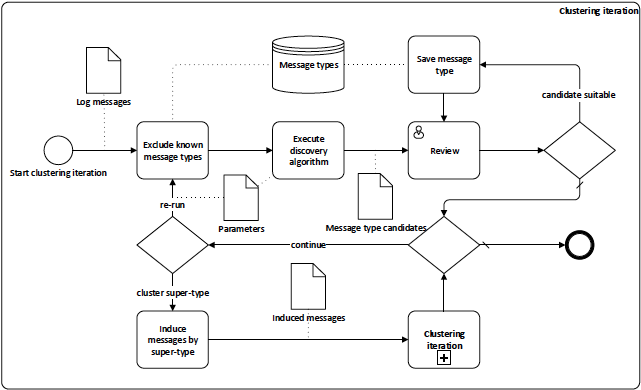
\includegraphics[width=\textwidth]{images/RURC.png} 	
 \end{minipage}
  \caption{ERD diagram vzorov}
  \label{fig:erd-patterns}
\end{figure}

\subsection{Prevod medzi formátmi parsovacích vzorov}
\label{sec:format-transformation}

Pri prevode medzi týmito formátmi potrebujeme mať vopred známu sadu typov regulárnych výrazov, voči ktorým budeme konverziu prevádzať. Je žiadúce, aby táto sada nebola konštantná pre všetky parsovacie vzory, ale aby bolo možné ju zadať pre vybrané parsovacie vzory. Z tohto dôvodu nie je transformácia medzi formátmi prevádzaná pri uložení parsovacieho vzoru, ale je vykonaná on demand pre zadanú sadu typov algoritmom \ref{fig:pattern-transformation}.

\begin{figure}[htbp]
\centering
\begin{minipage}{0.9\textwidth}
\lstset{tabsize=4,columns=flexible,breaklines=true,breakatwhitespace=true, showstringspaces=false}
\begin{lstlisting}
def transform_pattern_to_regex(pattern, pattern_lines, regex_types):
    types_tab = build_pattern_types_tab(pattern, pattern_lines, regex_types)

    transformed_patterns = {}
    pattern_idx = 0
    for line_key, types in types_tab.items():

        idx = 0
        replacements = []
        replacement = ''
        for words_in_groups in line_key.split():
            replacement = ''
            for words_in_group in words_in_groups:
                replacement.append('%{{{name}:var{idx}}}'.format(name=types[idx], idx=idx))
                idx += idx
            replacements.append(replacement)
            
        transformed_patterns['pattern' + pattern_idx] = replace_groups_text(pattern, replacements)

    return transformed_patterns


def build_pattern_types_tab(pattern, pattern_lines, regex_types):
    pattern_types = {}

    for line in pattern_lines:
        pattern_match = pattern.match(line)
        types = []
        keys = []
        pattern_groups = pattern_match.groups()
        for pattern_group in pattern_groups:
            words = pattern_group.split()
            for word in words:
                types.append(find_first_suitable_regex_type(word, regex_types))
            keys.append(str(len(words)))
        line_key = ','.join(keys)
        update_types(pattern_types, line_key, types)

    return pattern_types
\end{lstlisting} 		
\end{minipage} 
\caption{Databázovy model typu Source}
\label{fig:pattern-transformation}
\end{figure}

Hlavný rozdiel medzi popisovanými formátmi je ten, že pokým nativný formát algoritmu Extended Naggap-Vouk skracuje výskyt viacerých parametrov v rade, REtrie formát tento zápis nepozná. Preto vo výsledku z jedného parsovacieho vzoru môže vzniknúť až 

\begin{align*}
\prod_{group \in groups} group.upper\_bound - group.lower\_bound
\end{align*}

nových vzorov. Ďalší rozdiel je neprítomnosť typu parametra v pôvodnom formáte.
